\newpage
\section{Virtual Memory}

\subsection{Background}
Virtual memory -- separation of user logical memory from physical memory.

仅仅一部分在 memory 的程序需要运行. 所以逻辑内存可以大于物理内存. 甚至可以把虚地址扩展到和外存一样大. 

\begin{definition}
    Virtual memory isn't a physical object, but refers to the collection of abstractions and mechanisms the kernel provides to manage physical memory and virtual addresses.(Xv6 book)
\end{definition}

\begin{figure}[!htb]
    \centering
    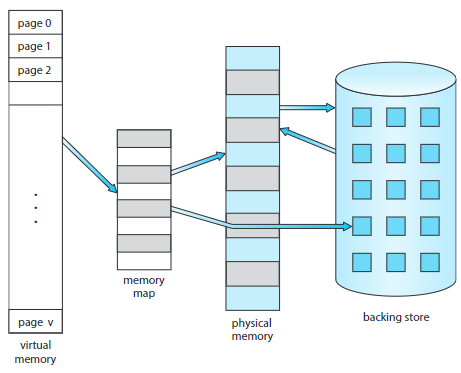
\includegraphics[width=0.42\textwidth]{pic/OS9/Diagram showing virtual memory that is larger than physical memory}
    \caption{Diagram showing virtual memory that is larger than physical memory}
\end{figure}

\begin{figure}[!htb]
    \centering
    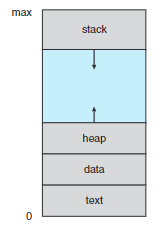
\includegraphics[width=0.16\textwidth]{pic/OS9/Virtual address space of a process in memory}
    \caption{Virtual address space of a process in memory}
\end{figure}

Other benefits:
\begin{itemize}
    \item 动态链接
    \item 共享内存
    \item 共享 page
\end{itemize}


\subsection{Demand Paging(请求式调页)}
Bring a page into memory only when it is needed. 

Lazy swapper -- never swaps a page into memory unless page will be needed. Swapper that deals with pages is a pager.

与之相对的是 eager swapper, 会预取. 

Transfer of a Paged Memory to Contiguous Disk Space. swap 连续的 memory. 

\subsubsection{Valid-Invalid Bit}
With each page table entry a valid–invalid bit is associated
\begin{itemize}
    \item v: in memory
    \item i: not in memory
\end{itemize}
save in table, called another table

\subsubsection{Page Fault}
If there is a reference to a page, first reference to that page will trap to operating system: page fault
\begin{enumerate}
    \item Operating system looks at another table (kept with PCB)
    to decide:
    \subitem Invalid reference $\to$ abort
    \subitem Just not in memory
    \item Get empty frame
    \item Swap page into frame
    \item Reset tables
    \item Set validation bit = v
    \item Restart the instruction that caused the page fault
\end{enumerate}

但会有问题: block move

\subsubsection{A Page Fault Causes The Following}
\begin{enumerate}%TODO 16
    \item 
\end{enumerate}

\begin{figure}[!htb]
    \centering
    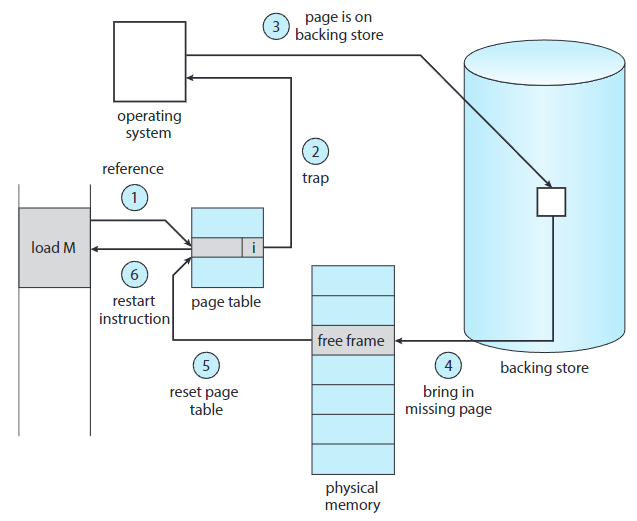
\includegraphics[width=0.42\textwidth]{pic/OS9/Steps in handling a page fault}
    \caption{Steps in handling a page fault}
\end{figure}


\subsubsection{Performance of Demand Paging}
Page Fault Rate: $0\le p \le 1$

Effective Access Time (EAT)
\begin{align*}
    EAT =& (1-p)\times \text{memory access}\\
        & + p \left( \begin{array}{rl}
              &\text{page fault overhead}\\
            + &\text{swap page out}\\
            + &\text{swap page in}\\
            + &\text{restart overhead}
        \end{array} \right)
\end{align*}

\subsection*{Process Creation}
Virtual memory allows other benefits during process creation
\begin{itemize}
    \item Copy-on-Write
    \item Memory-Mapped Files
\end{itemize}

\subsection{Copy-on-Write}
Copy-on-Write (COW) allows both parent and child processes to initially share the same pages in memory.Free pages are allocated from a pool of zeroed-out pages. 

\begin{figure}[!htb]
    \centering
    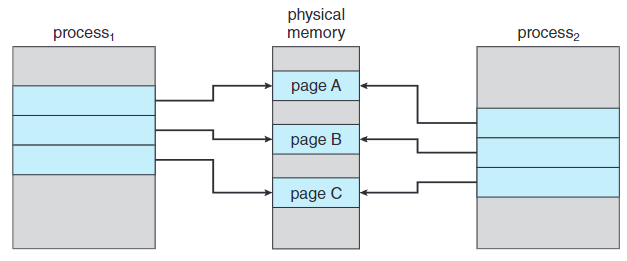
\includegraphics[width=0.42\textwidth]{pic/OS9/Before process 1 modifies page C}
    \caption{Before process 1 modifies page C}
\end{figure}

\begin{figure}[!htb]
    \centering
    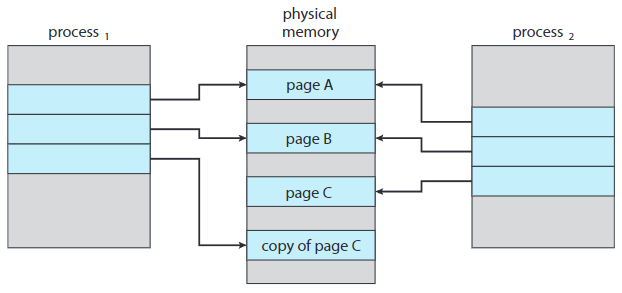
\includegraphics[width=0.42\textwidth]{pic/OS9/After process 1 modifies page C}
    \caption{After process 1 modifies page C}
\end{figure}

\subsection{Page Replacement}
If there is no free frame: Page replacement -- find some page in memory, but not really in use, swap it out. 

\begin{figure}[!htb]
    \centering
    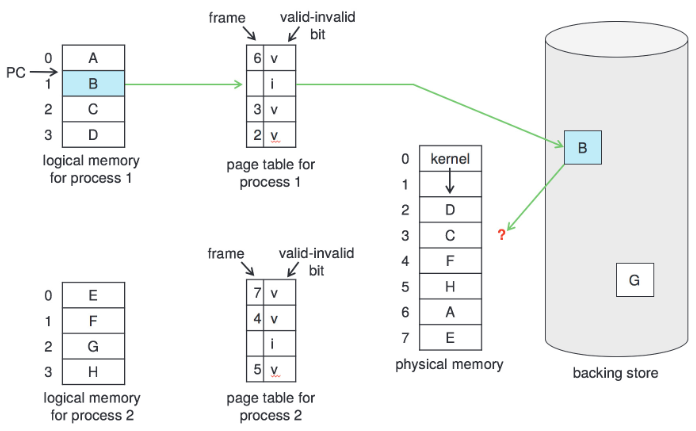
\includegraphics[width=0.42\textwidth]{pic/OS9/Need for page replacement}
    \caption{Need for page replacement}
\end{figure}

\subsubsection{Basic Page Replacement}
\begin{enumerate}\small
    \item Find the location of the desired page on secondary
    storage.
    \item Find a free frame:
    \begin{itemize}\scriptsize
        \item If there is a free frame, use it.
        \item If there is no free frame, use a page-replacement
        algorithm to select a victim frame.
        \item Write the victim frame to secondary storage (if
        necessary); change the page and frame tables
        accordingly. (Use dirty bit)
    \end{itemize}
    \item Read the desired page into the newly freed frame;
    change the page and frame tables.
    \item Continue the process from where the page fault
    occurred.
\end{enumerate}

\begin{figure}[!htb]
    \centering
    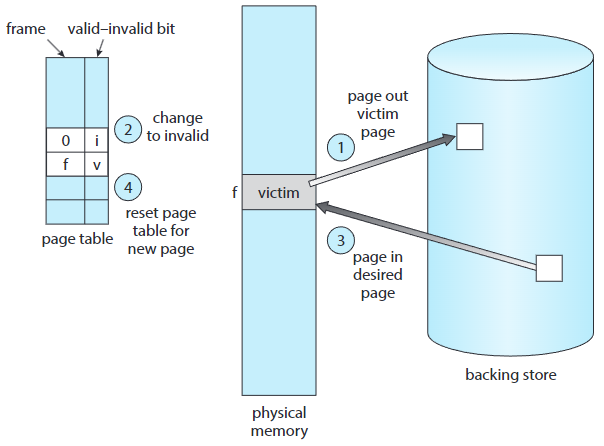
\includegraphics[width=0.42\textwidth]{pic/OS9/Page replacement}
    \caption{Page replacement}
\end{figure}

Page Replacement Algorithms: Want lowest page-fault rate. 

\subsubsection{First-In-First-Out (FIFO) Algorithm}
First-In-First-Out
\begin{figure}[!htb]
    \centering
    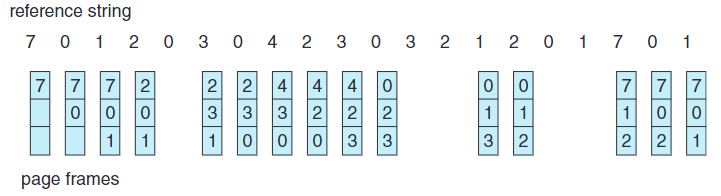
\includegraphics[width=0.42\textwidth]{pic/OS9/FIFO page-replacement algorithm}
    \caption{FIFO page-replacement algorithm}
\end{figure}

Belady's Anomaly: more frames $\Rightarrow$ more page faults. 

sequential flood. 

\subsubsection{Optimal Algorithm}
Replace page that will not be used for longest period of time. Just used for measuring how well your algorithm performs. 

\begin{figure}[!htb]
    \centering
    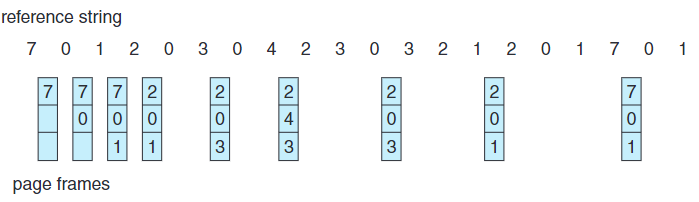
\includegraphics[width=0.42\textwidth]{pic/OS9/Optimal page-replacement algorithm}
    \caption{Optimal page-replacement algorithm}
\end{figure}

\subsubsection{Least Recently Used (LRU) Algorithm}
\begin{figure}[!htb]
    \centering
    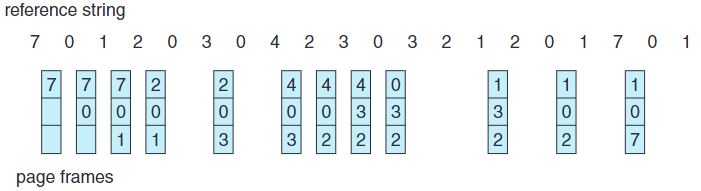
\includegraphics[width=0.42\textwidth]{pic/OS9/LRU page-replacement algorithm}
    \caption{LRU page-replacement algorithm}
\end{figure}

\begin{itemize}
    \item Counter implementation: write clock into counter, look at counters to determine which is to change. 
    \item Stack implementation: keep a stack of page numbers in a double
    link form. When Page referenced, move it to the top. 
\end{itemize}

\subsubsection{LRU Approximation Algorithms}
Reference bit: 
\begin{itemize}\scriptsize
    \item With each page associate a bit, initially = 0
    \item When page is referenced bit set to 1
    \item Replace the one which is 0 (if one exists)
\end{itemize}

Second chance: 
\begin{itemize}\scriptsize
    \item Need reference bit
    \item Clock replacement
    \item If page to be replaced (in clock order) has reference bit = 1
    then:
    \begin{itemize}
        \item set reference bit 0
        \item leave page in memory
        \item replace next page (in clock order), subject to same rules
    \end{itemize}
    \item 扫描, 若1则置0, 若0替换. 
\end{itemize}

\begin{figure}[!htb]
    \centering
    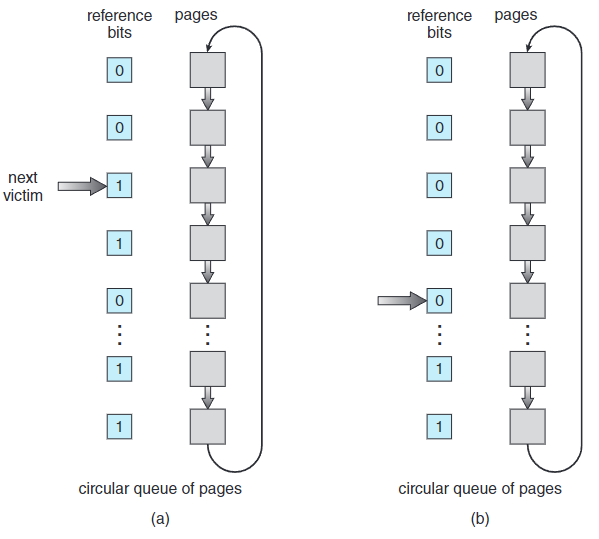
\includegraphics[width=0.42\textwidth]{pic/OS9/Second-chance (clock) page-replacement algorithm}
    \caption{Second-chance (clock) page-replacement algorithm}
\end{figure}

\subsubsection{Counting-based Algorithms}
Keep a counter of the number of references that have been made to each page


Other: 
\begin{itemize}\scriptsize
    \item LFU Algorithm: replaces page with smallest count
    \item MFU Algorithm: based on the argument that the page with the smallest count was probably just brought in and has yet to be used
\end{itemize}

\subsection{Allocation of Frames}
Each process needs minimum number of pages --- usually determined by computer architecture

Two major allocation schemes:
\begin{itemize}
    \item fixed allocation
    \begin{itemize}\scriptsize
        \item Equal allocation
        \item Proportional allocation - Allocate according to the size of process
    \end{itemize}
    \item priority allocation
    \subitem Use a proportional allocation scheme using priorities rather than size
\end{itemize}

\subsubsection{Global vs. Local Allocation}
\begin{itemize}%TODO 45
    \item Global replacement
    \item Local replacement
\end{itemize}

\subsection{Thrashing(颠簸)}
Thrashing: a process is busy swapping pages in and out. 

Total size of locality > total memory size
\begin{figure}[!htb]
    \centering
    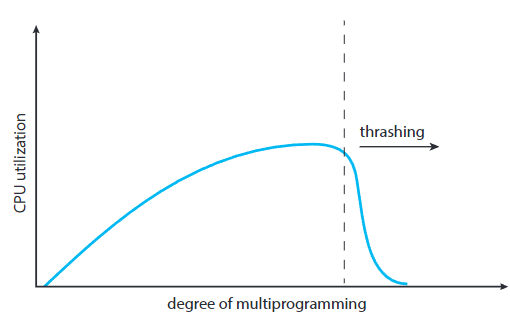
\includegraphics[width=0.309\textwidth]{pic/OS9/Thrashing}
    \caption{Thrashing}
\end{figure}

To limit the effect of thrashing: local replacement algo cannot
steal frames from other processes. But queue in page device
increases effective access time.

To prevent thrashing: allocate memory to accommodate its
locality

\subsubsection{Working-Set Model}
Let $\Delta$ be working-set window, which is a fixed number of page references. 

$WSS_i(\text{working-set size of Process }P_i)=$ total number of pages referenced in the most recent $\Delta$ (varies in time). 

Let $D=\sum WSS_i$ be total demand frames for all processes in the system. If $D>m$, thrashing, then suspend one of the processes. 

\subsubsection{Keeping Track of the Working Set}
Approximate with interval timer + a reference bit. 

e.g. %TODO 53

\begin{figure}[!htb]
    \centering
    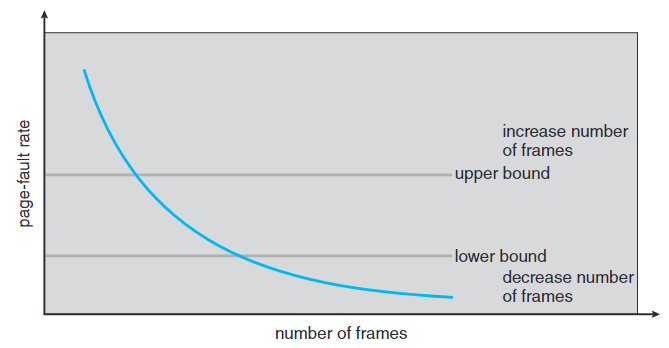
\includegraphics[width=0.309\textwidth]{pic/OS9/Page-fault frequency}
    \caption{Page-fault frequency}
\end{figure}



\subsection{Memory-Mapped Files}
%TODO 55-57

\subsection{Allocating Kernel Memory}
Often allocated from a free-memory pool

\subsubsection{Buddy System}
Allocates memory from fixed-size segment consisting of physically- contiguous pages

Memory allocated using power-of-2 allocator. 

\begin{figure}[!htb]
    \centering
    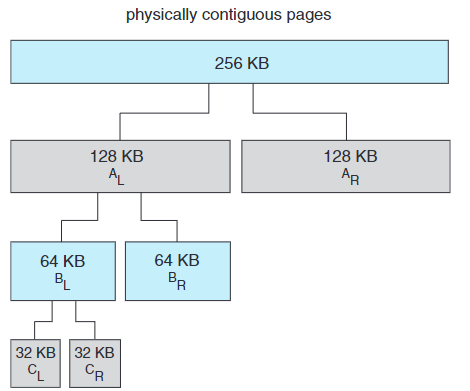
\includegraphics[width=0.309\textwidth]{pic/OS9/Buddy system allocation}
    \caption{Buddy system allocation}
\end{figure}

\subsubsection{Slab Allocator}
Slab is one or more physically contiguous pages. Cache consists of one or more slabs.  Each cache filled with objects -- instantiations of the data
structure

\begin{figure}[!htb]
    \centering
    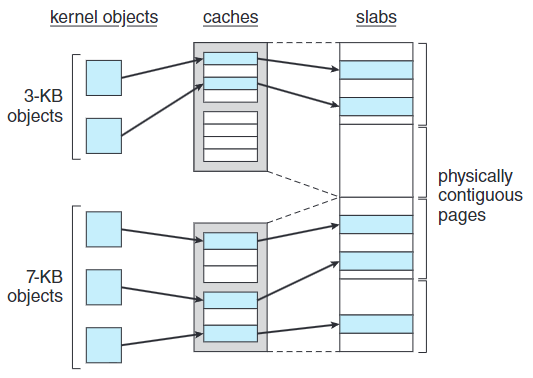
\includegraphics[width=0.42\textwidth]{pic/OS9/Slab allocation}
    \caption{Slab allocation}
\end{figure}


\subsection{Other Issues}
\subsubsection{Prepaging/Prefetching}
To reduce the large number of page faults that occurs at process startup
%TODO P63

\subsubsection{Page Size}
Page size selection must take into consideration

%TODO P64

\subsubsection{TLB Reach}
%TODO 65

\subsubsection{Program Structure}
%TODO P66

% \subsection{Operating-System Examples}